\documentclass{beamer}
\usepackage{amssymb}
\usepackage{tikz-cd}

\usetikzlibrary{decorations.pathmorphing}

\newcommand{\p}{\mathfrak{p}}
\newcommand{\Q}{\mathbb{Q}}
\newcommand{\Z}{\mathbb{Z}}
\newcommand{\F}{\mathbb{F}}
\newcommand{\PP}{\mathbb{P}}
\newcommand{\OO}{\mathcal{O}}
\newcommand{\Gal}{{\rm Gal}}
\newcommand{\pnorm}[1]{\left| #1 \right|_p}
\newcommand{\fnorm}[3]{{\rm N}^{#1}_{#2}\left( #3 \right)}
% \usepackage{../../commands}
\usetheme{Madrid}
% \usecolortheme{beaver}
%Information to be included in the title page:
\title{Galois Groups of Trinomials with Small \\ Coefficients}
\author{Hilel Garmi}
% \institute{Overleaf}
\date{2026}

\begin{document}

\frame{\titlepage}

\begin{frame}
    \frametitle{Main Example}
    \begin{alertblock}{}
        $$x^n - 2x + 1$$
    \end{alertblock}
\end{frame}

\begin{frame}
    \frametitle{Motivation}
    \only<1-3>{
        \begin{alertblock}{Hilbert's Irreducibility Theorem (1892)}
            For "almost" any polynomial $f \in \Q[x]$ of degree $n$, $\Gal(f) = S_n$.
        \end{alertblock}
    }
    \begin{alertblock}<2->{Schur (1931)}
        The Galois group of 
        \[
            f =\sum_{k=0}^n \binom{n}{k} \frac{x^k}{k!}
        \]
        is $S_n$ for all $n \geq 1$.
    \end{alertblock}
    \begin{alertblock}<3->{Nart \& Vila (1979) }
        The Galois group of $x^n - x- 1$ is $S_n$ for all $n \geq 2$.
    \end{alertblock}
    \begin{alertblock}<4->{Bary-Soroker \& Kozma (2020) }
        If we sample the coefficients of a monic polynomial of degree $n$ uniformly and independently from $\left\{ 1,\dots,210 \right\}$ then $\PP\left( \Gal\left( f \right) \in \left\{ A_n, S_n \right\} \right) \underset{n \to \infty}{\longrightarrow} 1$.
    \end{alertblock}
\end{frame}

\begin{frame}[fragile]
    \frametitle{Inertia Groups}
    \only<1-7>{
        \begin{block}{Notation}
            \only<2->{For any field $\F$, }
            \begin{itemize}
                \item<2-> Let $\overline{\F}$ be an algebraic closure of $\F$.
                \item<3-> Let $G_\F := \Gal\left( \overline{\F} / \F \right)$ be its absolute Galois group. 
            \end{itemize}
        \end{block}
    }
    \only<4->{
        \begin{block}{}
            \begin{columns}
                \begin{column}{8 cm}
                    \[
                        \begin{tikzcd}[ampersand replacement=\&]
                            \only<4-9>{
                                0 \arrow[r] \& p\Z_p \arrow[r] \& \Z_p \arrow[r] \& \F_p \arrow[r] \& 0
                            }
                            \only<5-9>{ \\ 
                                0 \arrow[r] \& \p \arrow[r] \& \OO_L \arrow[r] \& \F_q \arrow[r] \& 0
                            }
                            \only<6-12>{ \\ 
                                0 \arrow[r] \& \p \arrow[r] \& \OO_{\overline{\Q_p}} \arrow[r] \& \overline{\F_p} \arrow[r] \& 0
                            }
                            \only<8-14>{ \\
                                \& \& \overline{\Q_p} \arrow[d, "\sigma"{name=L}] \& \only<9-14> {\overline{\F_p} \arrow[d, "\overline{\sigma}"'{name=R}]}\& \\
                                \& \& \overline{\Q_p} \& \only<9-14> {\overline{\F_p}} \&
                                \only<9-14>{
                                    \arrow[rightarrow, from=L, to=R, squiggly, shorten <=2pt]
                                }
                            }
                            \only<10->{ \\
                                \only<11->{1 \arrow[r]}\& \only<11->{I_{\Q_p} \arrow[r]} \& G_{\Q_p} \arrow[r] \& G_{\F_p} \&
                            }
                        \end{tikzcd}
                    \]
                    \only<12->{
                        \[
                            f''\left( x \right) = n\left( n-1 \right) x^{n-2}
                        \]
                    }
                \end{column}
                \begin{column}{4 cm}
                    \only<7->{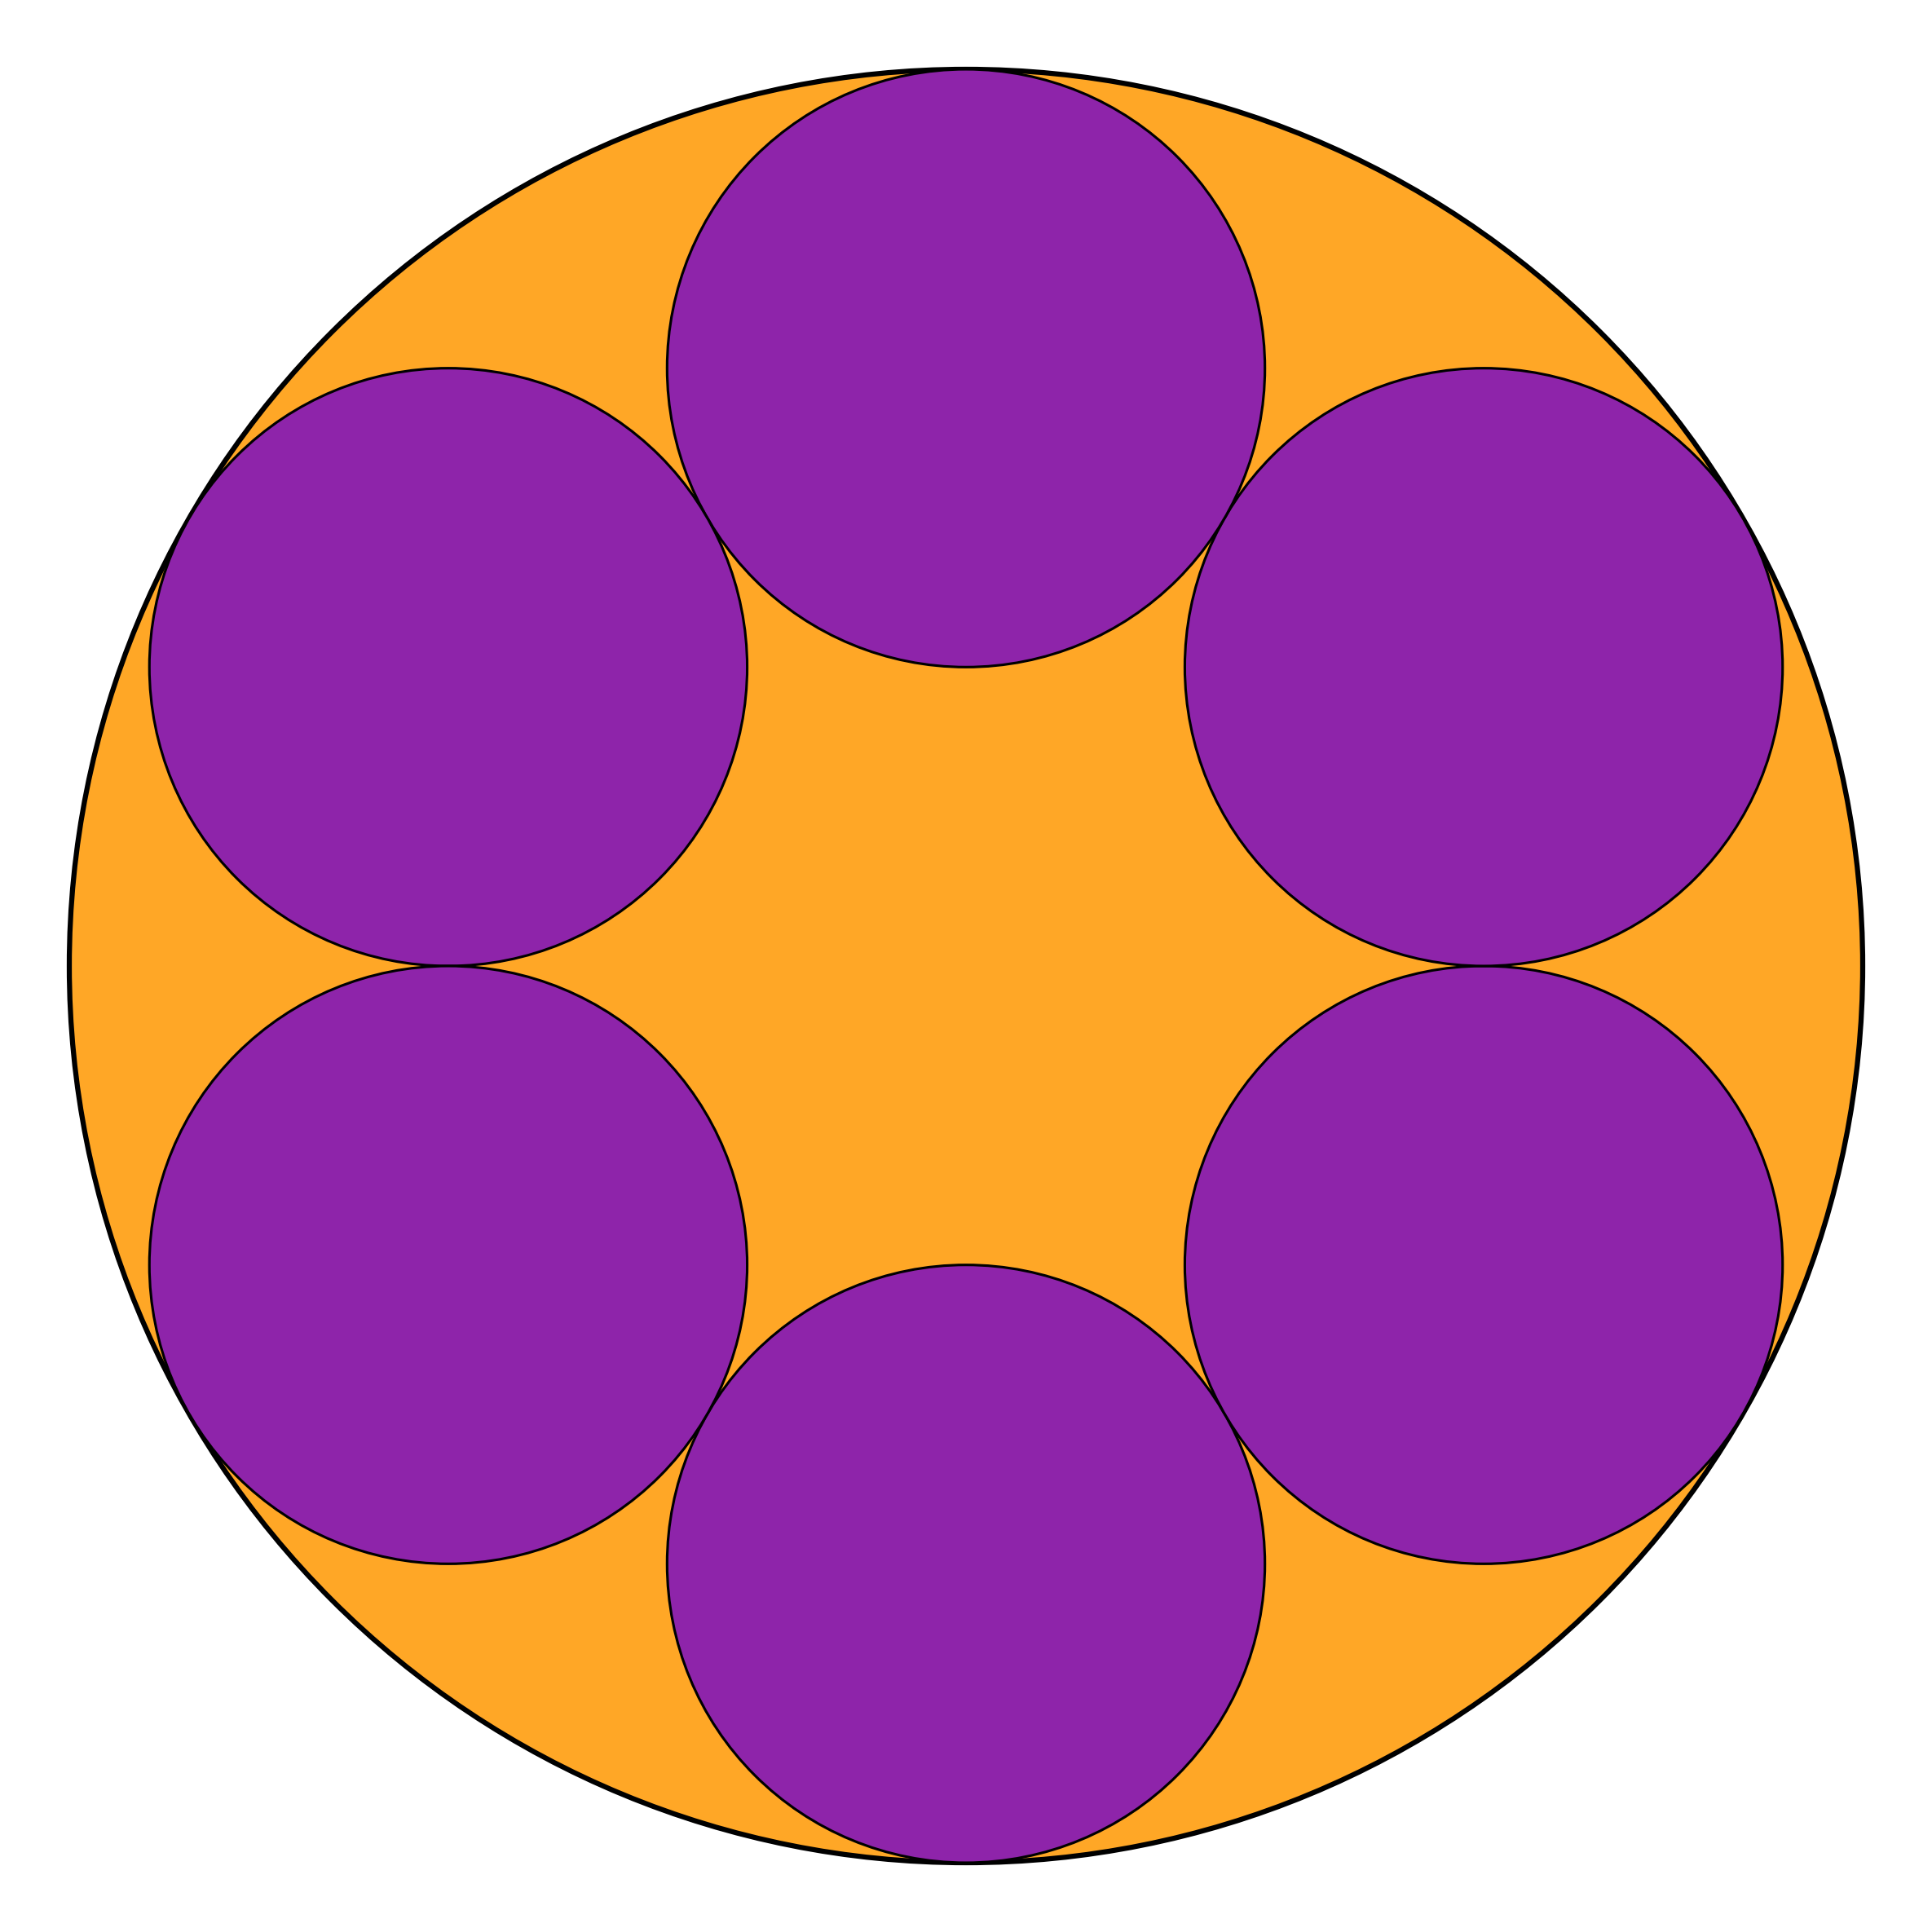
\includegraphics[height=4cm]{Zp.png}}
                \end{column}
            \end{columns}
        \end{block}
    }
    \only<13->{
        \begin{block}{}
            For any primes $p$: 
            
            \begin{itemize}
                \item<14->
                $f$ has no triple roots and at most one double root in $\overline{\F_p}$. 
                \only<15-> {$\Longrightarrow$}
                \item<15-> $I_{\Q_p}$ acts on the roots of $f$ either trivially or as a single transposition. 
            \end{itemize}
        \end{block}
    }
\end{frame}

% \begin{frame}

% \end{frame}

\end{document}